

\begin{frame}
\frametitle{Transformada Wavelet Discreta I}

\small
Si elegimos un subconjunto de desplazamientos $b$ y escala $a$ adecuados podemos obtener una base ortonormal de wavelets y realizar  una descomposici\'{o}n de la se\~{n}al en diferentes niveles:

\begin{columns}[t]
\begin{column}{4.5cm}

\footnotesize

\begin{itemize}
\item $\psi(\frac{t-b}{a})$
\item $a=2^l$ con $l \in \mathcal{ I}$
\item $b=k\cdot 2^l$ con $k \in \mathcal{ I}$
\item $\psi(\frac{t-\cdot 2^l k}{2^l})=\psi(2^{-l}t-k)$

\end{itemize}

\end{column}
\hspace{-1.5cm}\begin{column}{5cm}

\vspace{-0.5cm}



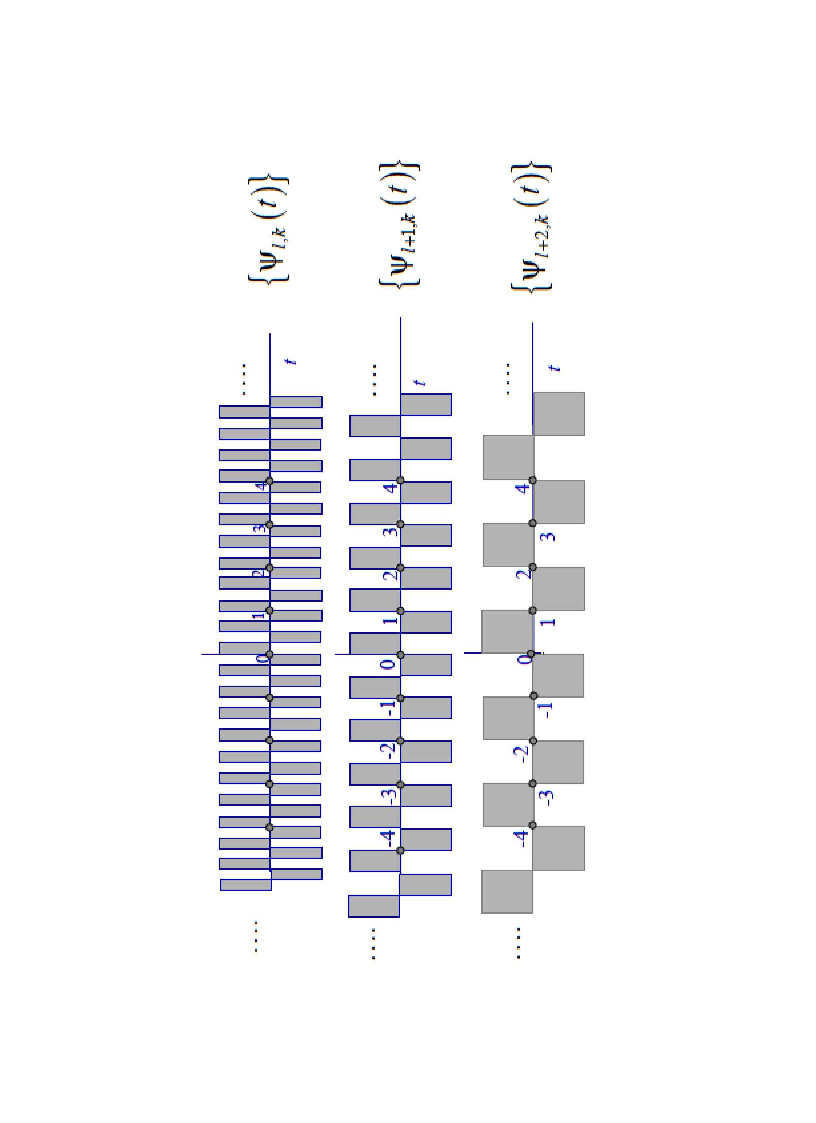
\includegraphics[width=3.cm,trim={5.5cm 5.5cm 5.5cm 4cm},clip,angle=-90]{./Figures/basewave}
\end{column}

\end{columns}

\visible<2->{

\begin{columns}[t]
\begin{column}{12cm}

\begin{itemize}

\footnotesize

 \vspace{-0.2cm}

\item Son una base ortonormal: $\int_{-\infty}^\infty \psi_{l_1,k_1}(t) \psi_{l_2,k_2}(t) = \delta(l_1-l_2)(\delta(k_1-k_2) $



\end{itemize}

\end{column}

\end{columns}

\vspace{0.0cm}

\begin{columns}[t]
\vspace{-0.5cm}\begin{column}{5cm}

\footnotesize

  \visible<3->{

\color{gray}

\textit{Se aplican sobre se\~{n}ales continuas con desplazamientos y escalados discretos.  }


\textit{Tambi\'{e}n existen definiciones para variables discretas y para secuencias finitas.  }}


\end{column}

\vspace{-0.2cm}\begin{column}{5cm}

\vspace{-0.2cm}

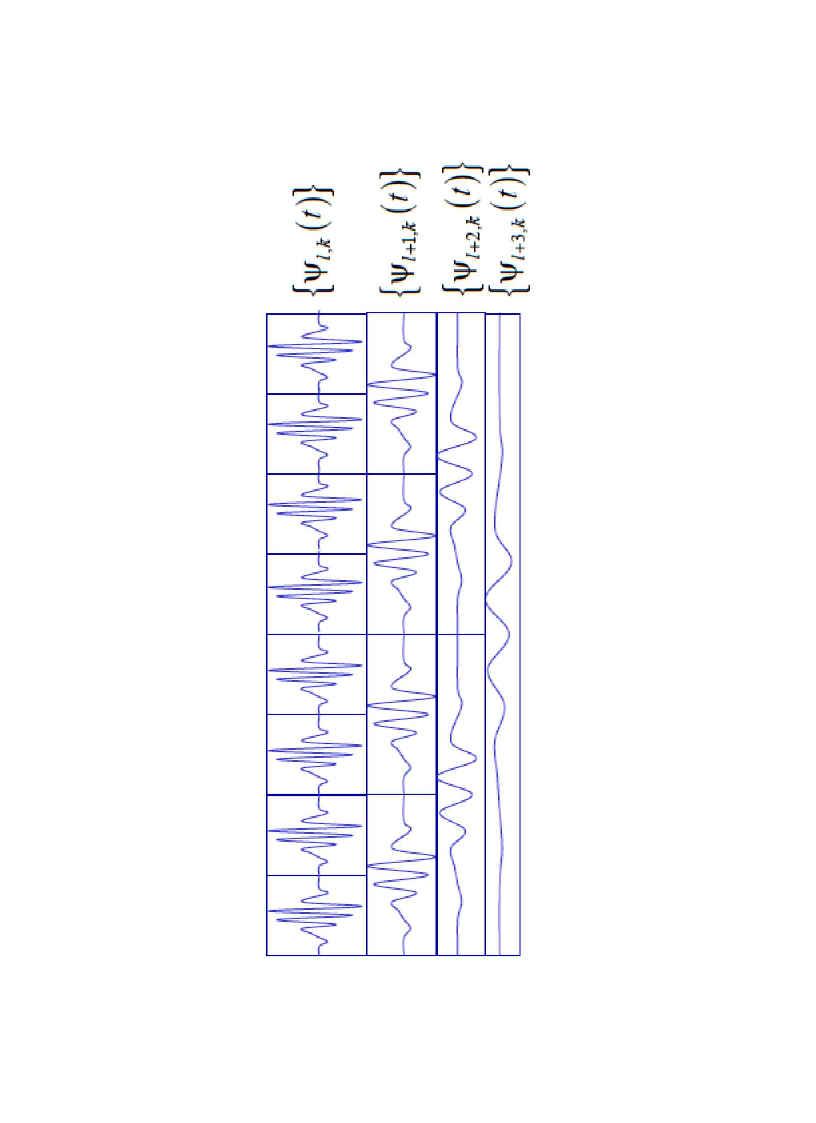
\includegraphics[width=2.2cm,trim={7.0cm 4.0cm 5.5cm 4cm},clip,angle=-90]{./Figures/basewave2}

\end{column}

\end{columns}}


\end{frame}

\begin{frame}
\frametitle{Transformada Wavelet Discreta II}

\begin{itemize}

\item Matlab (moodle): \color{red}dwtplot(y,nlevels,'waveletname') \color{black}

\vspace{0.1cm}

\color{red} y: \color{black} vector de valores

\vspace{0.1cm}


\color{red} nlevels: \color{black} numero de niveles

\vspace{0.1cm}


\color{red} 'waveletname': \color{black} nombre de la wavelet

\end{itemize}


\vspace{0.1cm}

\visible<2->{

\color{olivegreen} Ejemplo: \color{black}  Calcular la wavelet de $y(t)=1-| \frac{t-50}{50} |$

\begin{columns}[t]

\begin{column}{5.0cm}




\lstinputlisting{./Matlab/waveletdiscreta1.m}

\end{column}


\begin{column}{5.5cm}

\includegraphics[width=5.5cm]{./Figures/waved1.eps}



\end{column}





\end{columns}}


\end{frame}


\begin{frame}
\frametitle{Transformada Wavelet Discreta III}

\vspace{-0.2cm}

\color{red}
Descomposici\'{o}n por niveles de la se\~{n}al:\color{black}

\vspace{-0.1cm}

\small

\begin{itemize}
\item Coeficientes wavelet: $X(l,k)=\int_{-\infty}^{\infty} \psi_{l,k}(t)x(t)dt$

\item Reconstruccion se\~{n}al: $\displaystyle x(t)=\sum_{l=-\infty}^\infty \sum_{k=-\infty}^\infty X(l,k) \psi_{l,k}(t)$


\visible<2->{
\vspace{-0.1cm}

\item Grado de detalle de un nivel: $\displaystyle D_l(t)=\sum_{k=-\infty}^\infty X(l,k) \psi_{l,k}(t)$}

\visible<3->{

\vspace{-0.5cm}

\item Se\~{n}al original: $\displaystyle f(t)=\sum_{l=-\infty}^\infty D_l(t)$}

\vspace{-0.4cm}

\visible<4->{
\item Aproximaci\'{o}n a partir del nivel umbral $J$: $\displaystyle A_J(t)=\sum_{l=J+1}^\infty D_l(t)$

\footnotesize Mantiene la parte de se\~{n}al sin los detalles de escalas m\'{a}s peque\~nas.}

\small

\vspace{-0.2cm}

\visible<5->{

\item Se\~{n}al original: $\displaystyle f(t)=\sum_{l=-\infty}^J D_l(t)+ A_J(t)$}

\vspace{-0.1cm}

\visible<6->{
\item $A_{J-1}(t)=\sum_{l=J}^\infty D_l(t)=D_J(t)+\sum_{l=J+1}^\infty D_l(t)=D_J(t)+A_{J}(t)$}

\visible<7->{

\item $D_l(t)$ se obtiene integrando con $\psi_{l,k}(t)$}

\visible<8->{
\item  $A_l(t)$ se obtiene de lo que queda, o de la wavelet `padre' $\phi_{l,k}(t)$}


\end{itemize}



\end{frame}


\begin{frame}
\frametitle{Transformada Wavelet Discreta IV}



\color{red}
Descomposici\'{o}n por niveles de la se\~{n}al:\color{black}

\centering
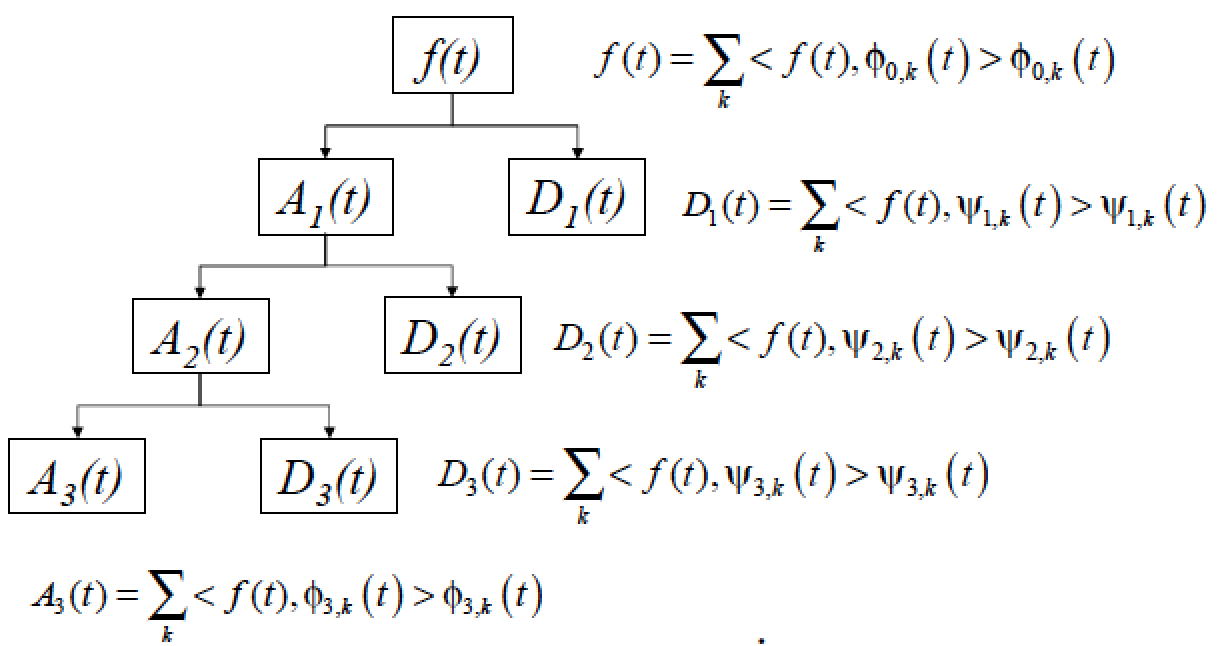
\includegraphics[width=9cm]{./Figures/Descomposicion}


\end{frame}

\begin{frame}
\frametitle{Transformada Wavelet Discreta V}


\vspace{-0.2cm}

\small

\color{red}
Descomposici\'{o}n por niveles de la se\~{n}al:\color{black}

\vspace{-0.2cm}

\begin{itemize}
\item Matlab: \color{red} [cA,cD]=dwt(f,'waveletname');

%\vspace{0.05cm}

\color{red}f \color{black}: se\~{n}al discretizada (coeficientes de la aproximaci\'{o}n del nivel anterior)

%\vspace{0.05cm}

\color{red} cD: \color{black} Coeficientes de wavelet para el nivel siguiente

%\vspace{0.05cm}

\color{red} cA: \color{black} Coeficientes de funci\'{o}n de escala del nivel siguiente

%\vspace{0.05cm}

\item Matlab (funci\'{o}n inversa): \color{red} f=idwt(cA,cD,'waveletname'); \color{black}


\footnotesize
\color{gray}\textit{Haciendo cero cada parte, puedo descomponer la se\~{n}al en las dos partes.}

\end{itemize}

\vspace{-0.5cm}

\visible<2->{

\begin{columns}[t]
\begin{column}{5cm}

\vspace{-0.4cm}

\lstinputlisting{./Matlab/waveletdiscreta2.m}




\end{column}


\begin{column}{5cm}

\includegraphics[width=4.5cm]{./Figures/waved2.eps}



\end{column}

\end{columns}

\scriptsize

\vspace{0.1cm}

\color{blue}\textit{
El n\'{u}mero de valores  en cada nivel se reduce
}}

\end{frame}


\begin{frame}
\frametitle{Transformada Wavelet Discreta VI}


\vspace{-0.2cm}

\small

\color{red}
Descomposici\'{o}n por niveles de la se\~{n}al:\color{black}

\vspace{-0.2cm}

\begin{itemize}
\item Matlab: \color{red} [coef,sl]=wavedec(f,niveles,'waveletname');

\hspace{1cm} values=wrcoef(tipo,coef,sl,'waveletname',nivel);

%\vspace{0.05cm}

\color{red}f \color{black}: se\~{n}al discretizada

%\vspace{0.05cm}

\color{red} niveles: \color{black} numero de niveles

\color{red} tipo: 'a'  \color{black}  aproximaci\'{o}n, \color{red} 'd' \color{black} detalle

\color{red} nivel: \color{black} nivel seleccionado

\color{red} value: \color{black} aproximaci\'{o}n o detalle del nivel elegido


\end{itemize}

\vspace{-0.5cm}

\visible<2->{

\begin{columns}[t]
\begin{column}{5cm}

\vspace{-0.6cm}

\lstinputlisting{./Matlab/waveletdiscreta3.m}




\end{column}


\begin{column}{5cm}

\vspace{0.2cm}

\includegraphics[width=4.5cm]{./Figures/waved3.eps}



\end{column}

\end{columns}

\scriptsize

\vspace{-0.2cm}

\color{blue}\textit{
El n\'{u}mero de valores  en cada nivel se mantiene}}

\end{frame}


\begin{frame}
\frametitle{Transformada Wavelet}

\begin{itemize}

\item La elecci\'{o}n del tipo de wavelet depender\'{a} del tipo de an\'{a}lisis que se desea realizar. Podr\'{a} tenerse en cuenta tanto su forma como sus propiedades (por ejemplo momentos evanescentes que tiene).

\item La transformada wavelet tambi\'{e}n pueden ser analizadas desde la perspectiva del paso de una se\~{n}al por un banco de filtros.

\item Tambi\'{e}n existe una transformada r\'{a}pida de wavelets.

\end{itemize}

\end{frame}
